\let\negmedspace\undefined
\let\negthickspace\undefined
\documentclass[journal]{IEEEtran}
\usepackage[a5paper, margin=10mm, onecolumn]{geometry}
\usepackage{lmodern} % Ensure lmodern is loaded for pdflatex
\usepackage{tfrupee} % Include tfrupee package

\setlength{\headheight}{1cm} % Set the height of the header box
\setlength{\headsep}{0mm}     % Set the distance between the header box and the top of the text

\usepackage{gvv-book}
\usepackage{gvv}
\usepackage{cite}
\usepackage{amsmath,amssymb,amsfonts,amsthm}
\usepackage{algorithmic}
\usepackage{graphicx}
\usepackage{textcomp}
\usepackage{xcolor}
\usepackage{txfonts}
\usepackage{listings}
\usepackage{enumitem}
\usepackage{mathtools}
\usepackage{gensymb}
\usepackage{comment}
\usepackage[breaklinks=true]{hyperref}
\usepackage{tkz-euclide} 
\usepackage{listings}
\usepackage{gvv}                                        
\def\inputGnumericTable{}                                 
\usepackage[latin1]{inputenc}                                
\usepackage{color}                                            
\usepackage{array}                                            
\usepackage{longtable}                                       
\usepackage{calc}                                             
\usepackage{multirow}                                         
\usepackage{hhline}                                           
\usepackage{ifthen}                                           
\usepackage{lscape}
\setlength{\parindent}{0pt}
\begin{document}

\bibliographystyle{IEEEtran}
\vspace{3cm}

\title{1.1.2.13}
\author{AI24BTECH11020 - RISHIKA KOTHA}
% \maketitle
% \newpage
% \bigskip
{\let\newpage\relax\maketitle}

\renewcommand{\thefigure}{\theenumi}
\renewcommand{\thetable}{\theenumi}
\setlength{\intextsep}{10pt} % Space between text and floats


\numberwithin{equation}{enumi}
\numberwithin{figure}{enumi}
\renewcommand{\thetable}{\theenumi}
\parindent 0px
Question:
The fourth vertex $\vec{D}$ of a parallelogram ABCD whose three vertices are $\vec{A}(-2, 3),\vec{B}(6, 7)$ and $\vec{C}(8, 3)$ is
\\
\solution

we know that, in a parallelogram,
\begin{align}
	                A+C&=B+D\\
	\implies	D&=A+C-B\\
	\implies        D&=\myvec{-2+8-6\\3+3-7}\\
	\therefore	D&=\myvec{0\\-1}
\end{align}
\begin{table}[h!]    
  \centering
  \begin{tabular}[12pt]{ |c| c| c|}
    \hline
	parameter & Description & value \\ 
    \hline
	 C & Centre & $\myvec{0\\ 13/6}$\\
    \hline 
	 O & point1 & $\myvec{0\\0}$\\
    \hline
	 P & point2 & $\myvec{2\\3}$\\
    \hline   
	 r & radius & 13/6\\
    \hline
    \end{tabular}

  \caption{Vertices}
  \label{tab1.2.13.1}
\end{table}

\begin{figure}[h!]
   \centering
   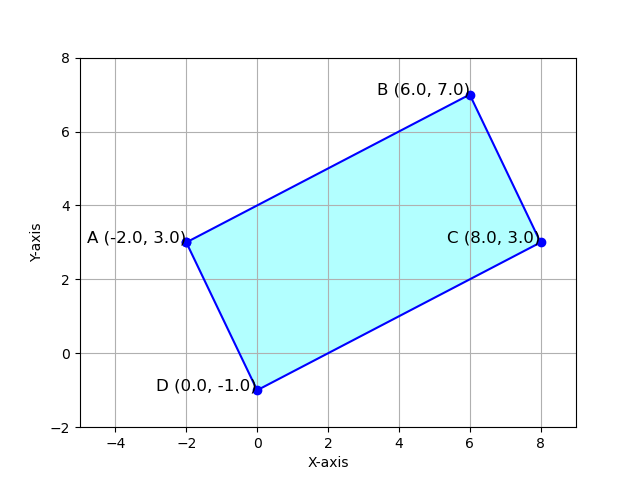
\includegraphics[width=0.7\columnwidth]{fig/Figure_1.png}
   \label{parallelogram graph}
\end{figure}

 \end{document}
